\section{Introduction}\label{introduction}

\subsection{Introduction}\label{introduction-1}

\begin{frame}{Introduction - 自我介绍}

\begin{itemize}
\itemsep1pt\parskip0pt\parsep0pt
\item
  American pediatrician - 美国儿科医生
\item
  Lived in China for 22 years - 在中国生活22年
\item
  Married for 28 years (prettiest surgeon in Northwest China!) -
  结婚28年(中国西北最美的外科医生)
\item
  Two daughters (23 and 17 years old) - 有两个女儿(一个23岁,一个17岁)
\end{itemize}

\end{frame}

\begin{frame}{Family - 家庭}

\begin{figure}
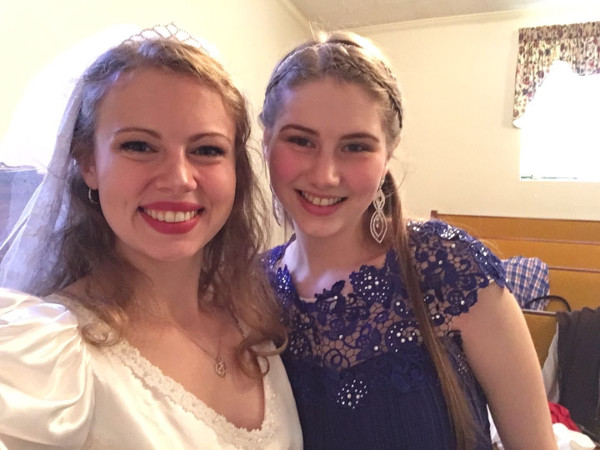
\includegraphics[scale=0.3]{./img/siblingsday.jpg}
\end{figure}

\end{frame}

\subsection{Objectives}\label{objectives}

\begin{frame}{Objectives}

\begin{itemize}
\itemsep1pt\parskip0pt\parsep0pt
\item
  Participants will understand the importance of thinking about the
  kidney when facing disease states such as diabetes, HSP and spina
  bifida.
\item
  Participants will develop a plan for first steps evaluation and
  nephroprotection in the above mentioned disease states.
\end{itemize}

\end{frame}

\subsection{Abstract}\label{abstract}

\begin{frame}{Abstract}

The kidney is affected by a variety of disease states. Some are
intrinsically renal in origin but many are not. The generalist can be
expected to see patients with diabetes, HSP or spina bifida in the
course of a normal practice. All of these affect the kidney in different
ways. This talk will cover the primary reno-protective measures a
primary care physician can employ to make sure the patient's kidney will
last as long as possible in these disease states.

\end{frame}

\section{Diabetes}\label{diabetes}

\frame{\tableofcontents[hideothersubsections]}

\subsection{Diabetes in Children}\label{diabetes-in-children}

\begin{frame}{Diabetes in children}

\begin{itemize}
\itemsep1pt\parskip0pt\parsep0pt
\item
  Obesity is increasingly becoming a disease of younger and younger
  people.
\item
  IDDM is most commonly linked to renal disease
\item
  NIDDM is increasing in adolescents
\item
  Proteinuria on urinalysis
\item
  No edema on physical exam
\end{itemize}

\end{frame}

\subsection{Clinical findings}\label{clinical-findings}

\begin{frame}{Microalbuminuria}

\begin{itemize}
\itemsep1pt\parskip0pt\parsep0pt
\item
  Can occur in both insulin and non-insulin dependent diabetes
\item
  Not massive proteinuria

  \begin{itemize}
  \itemsep1pt\parskip0pt\parsep0pt
  \item
    protein:creatinine is low (usually total of 30-300mg albumin/g
    creatinine)
  \item
    albumin is normal
  \end{itemize}
\item
  Due to protein leak at the tubule, not at the glomerulus
\item
  Slow decline in GFR, leads to CKD over years
\item
  Most patients present after years of diabetic disease - 15+
\end{itemize}

\end{frame}

\begin{frame}{Hematuria}

\begin{itemize}
\itemsep1pt\parskip0pt\parsep0pt
\item
  Unusual
\item
  When present, think glomerular leak
\item
  Adults have ticks and fleas - Think about other causes of renal
  disease - IgA, membranous, etc.
\item
  Biopsy shows mesangial proliferation, glomerular sclerosis
\end{itemize}

\end{frame}

\subsection{Renal protection}\label{renal-protection}

\begin{frame}{Renal protection}

\begin{itemize}
\itemsep1pt\parskip0pt\parsep0pt
\item
  Consider ACEI to protect the tubules
\item
  Monitor blood pressure and treat accordingly
\item
  Control diabetes to slow progression of renal disease

  \begin{itemize}
  \itemsep1pt\parskip0pt\parsep0pt
  \item
    Weight reduction
  \item
    Lipid control (rarely needed in peds)
  \end{itemize}
\item
  No protein restriction (in peds)
\end{itemize}

\end{frame}

\begin{frame}{Monitoring}

\begin{itemize}
\itemsep1pt\parskip0pt\parsep0pt
\item
  Yearly screens for proteinuria in all diabetics
\item
  q3 Month check of protein:creatinine ratio for patients with
  demonstrated proteinuria

  \begin{itemize}
  \itemsep1pt\parskip0pt\parsep0pt
  \item
    Goal is less than 1000mg/day protein excretion (less than 500 is
    even better!)
  \end{itemize}
\item
  Blood pressure monitoring
\item
  Follow potassium in patients on ACEI or ARB
\end{itemize}

\end{frame}

\section{IgA Vasculitis (HSP)}\label{iga-vasculitis-hsp}

\frame{\tableofcontents[hideothersubsections]}

\subsection{Presentation}\label{presentation}

\begin{frame}{Presentation}

\begin{itemize}
\itemsep1pt\parskip0pt\parsep0pt
\item
  Palpable purpura without thrombocytopenia
\item
  Arthritis/arthralgia
\item
  Abdominal pain
\item
  Renal disease
\end{itemize}

\end{frame}

\begin{frame}{IgAV Rash}

\begin{figure}
\includegraphics[scale=0.5]{./img/SknlsnHnchSchnlnprpIgA.jpg}
\end{figure}

\end{frame}

\begin{frame}{Dorsal hand edema}

\begin{figure}
\includegraphics[scale=0.5]{./img/IgAV_HSP_dorsal_edema_scale_crop.jpg}
\end{figure}

\end{frame}

\begin{frame}{Immunfluorescence}

\begin{figure}
\includegraphics[scale=0.5]{./img/IgA_nephropathy_IF.jpg}
\end{figure}

\end{frame}

\begin{frame}{Unusual manifestations}

\begin{itemize}
\itemsep1pt\parskip0pt\parsep0pt
\item
  Scrotal pain
\item
  Headache, seizures, encephalopathy
\item
  Respiratory signs
\item
  Keratitis and uveitis
\end{itemize}

\end{frame}

\subsection{Management}\label{management}

\begin{frame}{Management}

\begin{itemize}
\itemsep1pt\parskip0pt\parsep0pt
\item
  Maintain hydration, elevate edematous areas, etc.
\item
  Treat pain
\item
  Consider steroids
\item
  Hospitalize
\end{itemize}

\end{frame}

\begin{frame}{Outpatient management}

\begin{itemize}
\itemsep1pt\parskip0pt\parsep0pt
\item
  NSAIDS - naproxen or ibuprofen
\item
  Prednisone - rarely needed
\end{itemize}

\end{frame}

\begin{frame}{Criteria for hospitalization}

\begin{itemize}
\itemsep1pt\parskip0pt\parsep0pt
\item
  Unable to maintain hydration
\item
  Severe abdominal pain
\item
  GI bleeding
\item
  Mental status changes
\item
  Limited self-care (secondary to joint pain)
\item
  Renal insufficiency
\end{itemize}

\end{frame}

\begin{frame}{Monitoring}

\begin{itemize}
\itemsep1pt\parskip0pt\parsep0pt
\item
  1/3 or patients will recur at least once
\item
  Monitor urinalysis and BP weekly - q2w for the first 2 months after
  presentation
\item
  Monitor monthly until 1 year after initial presentation
\item
  Check BP and UA at annual well-child visits to monitor for adult
  disease onset
\end{itemize}

\end{frame}

\section{Myelomeningocele}\label{myelomeningocele}

\frame{\tableofcontents[hideothersubsections]}

\subsection{Case Study}\label{case-study}

\begin{frame}{A Case Study}

17YO African American female referred from Family Medicine clinic. Child
followed at state Spina Bifida clinic for her whole life. During routine
visit in the Family Medicine clinic she was discovered to have
hypertension. Investigation revealed a hematocrit of 17mg/dL, creatinine
of 9mg/dL. Family medicine resident immediately referred to peds
nephrology for evaluation and treatment.

\end{frame}

\begin{frame}{Varieties of neurogenic bladder}

\begin{itemize}
\itemsep1pt\parskip0pt\parsep0pt
\item
  Flaccid bladder
\item
  High pressure bladder
\item
  Hyperreflexic bladder
\item
  Overactive sphincter
\item
  Detrusor sphinctor dyssynergia
\end{itemize}

\end{frame}

\subsection{Assessment}\label{assessment}

\begin{frame}{Assessment}

\begin{itemize}
\itemsep1pt\parskip0pt\parsep0pt
\item
  Ultrasound of kidney and bladder
\item
  Urodynamics (voiding cystourethrogram, cystometrogram/EMG)
\item
  Consider DMSA/MAG3 renal scan
\item
  Urine culture
\end{itemize}

\end{frame}

\subsection{Management}\label{management-2}

\begin{frame}{Management - 4 Aspects}

\begin{itemize}
\itemsep1pt\parskip0pt\parsep0pt
\item
  Clean intermittent catheterization
\item
  Consider anticholinergics
\item
  UTIs
\item
  Bowel management
\end{itemize}

\end{frame}

\begin{frame}{Management - CIC}

\begin{itemize}
\itemsep1pt\parskip0pt\parsep0pt
\item
  Mainstay of therapy
\item
  Clean, not sterile
\item
  Start early (\textless{} 1YO)
\item
  Lanzhou approach != Alabama approach
\end{itemize}

\end{frame}

\begin{frame}{Management - Anticholinergics}

\begin{itemize}
\itemsep1pt\parskip0pt\parsep0pt
\item
  Oxybutynin (Ditropan)

  \begin{itemize}
  \itemsep1pt\parskip0pt\parsep0pt
  \item
    \textless{} 12m - 0.1mg/kg tid
  \item
    1-5YO 0.2mg/kg tid
  \item
    for \textgreater{} 5YO 5mg tabs tid, consider the transdermal
    preparation
  \end{itemize}
\item
  Tolterodine (Detrol)

  \begin{itemize}
  \itemsep1pt\parskip0pt\parsep0pt
  \item
    for \textgreater{} 5YO children
  \item
    1-2mg bid
  \end{itemize}
\item
  Both have long acting forms suitable for older children
\end{itemize}

\end{frame}

\begin{frame}{Management - UTI}

\begin{itemize}
\itemsep1pt\parskip0pt\parsep0pt
\item
  Cloudy, smelly urine

  \begin{itemize}
  \itemsep1pt\parskip0pt\parsep0pt
  \item
    Increase fluids
  \item
    Increase frequency of CIC
  \item
    Not necessarily a UTI
  \end{itemize}
\item
  UTI symptoms

  \begin{itemize}
  \itemsep1pt\parskip0pt\parsep0pt
  \item
    pain during CIC
  \item
    gross hematuria
  \item
    back or belly pain
  \item
    lethargy (think shunt malfunction too)
  \item
    fever (think about that shunt!)
  \item
    vomiting (more shunt worries)
  \end{itemize}
\end{itemize}

\end{frame}

\begin{frame}{Management - Bowel}

\begin{itemize}
\itemsep1pt\parskip0pt\parsep0pt
\item
  Neurogenic bowel a common co-morbidity
\item
  Most commonly constipated, may have laxity of anal sphincter
\item
  Goal of therapy is timed elimination, use laxatives, suppositories,
  enemas, etc.
\end{itemize}

\end{frame}

\section{Questions?}\label{questions}

\begin{frame}{Questions? 提问题?}

\begin{figure}[htbp]
\centering
\includegraphics{./img/img_0510_200.jpg}
\caption{}
\end{figure}

\end{frame}
